\documentclass[10pt]{article}
\usepackage{longtable}
\usepackage{float}
\usepackage{wrapfig}
\usepackage{rotating}
\usepackage[normalem]{ulem}
\usepackage{amsmath}
\usepackage{textcomp}
\usepackage{marvosym}
\usepackage{wasysym}
\usepackage{amssymb}
\usepackage{hyperref}
\usepackage{color,soul} % for highlighting
\usepackage{graphicx}
\graphicspath{{/Users/benjaminbass/seacloud/class/earthMaterials/picBank/}}

\usepackage{frame,color}
\usepackage{framed}
\usepackage{minibox}

% \usepackage[T1]{fontenc}
% \usepackage{tilting} %bring title up
% \setlength{\droptitle}{-10cm}

\usepackage[version=3]{mhchem}
% How to Use MChem
% \ce{SO4^2-}
% \ce{^{227}_{90}Th+}
% \ce{A\bond{-}B\bond{=}C\bond{#}D}
% \ce{CO2 + C -> 2CO}
% \ce{SO4^2- + Ba^2+ -> BaSO4 v}


\author{Benjamin Bass}
\date{15 March 2016}
\title{\vspace{-2.0cm} Tourmaline} %bring title up temporary Fix

\begin{document}

\maketitle

% \framebox{Use frameboxes until figure out alignmen}

\begin{center}
  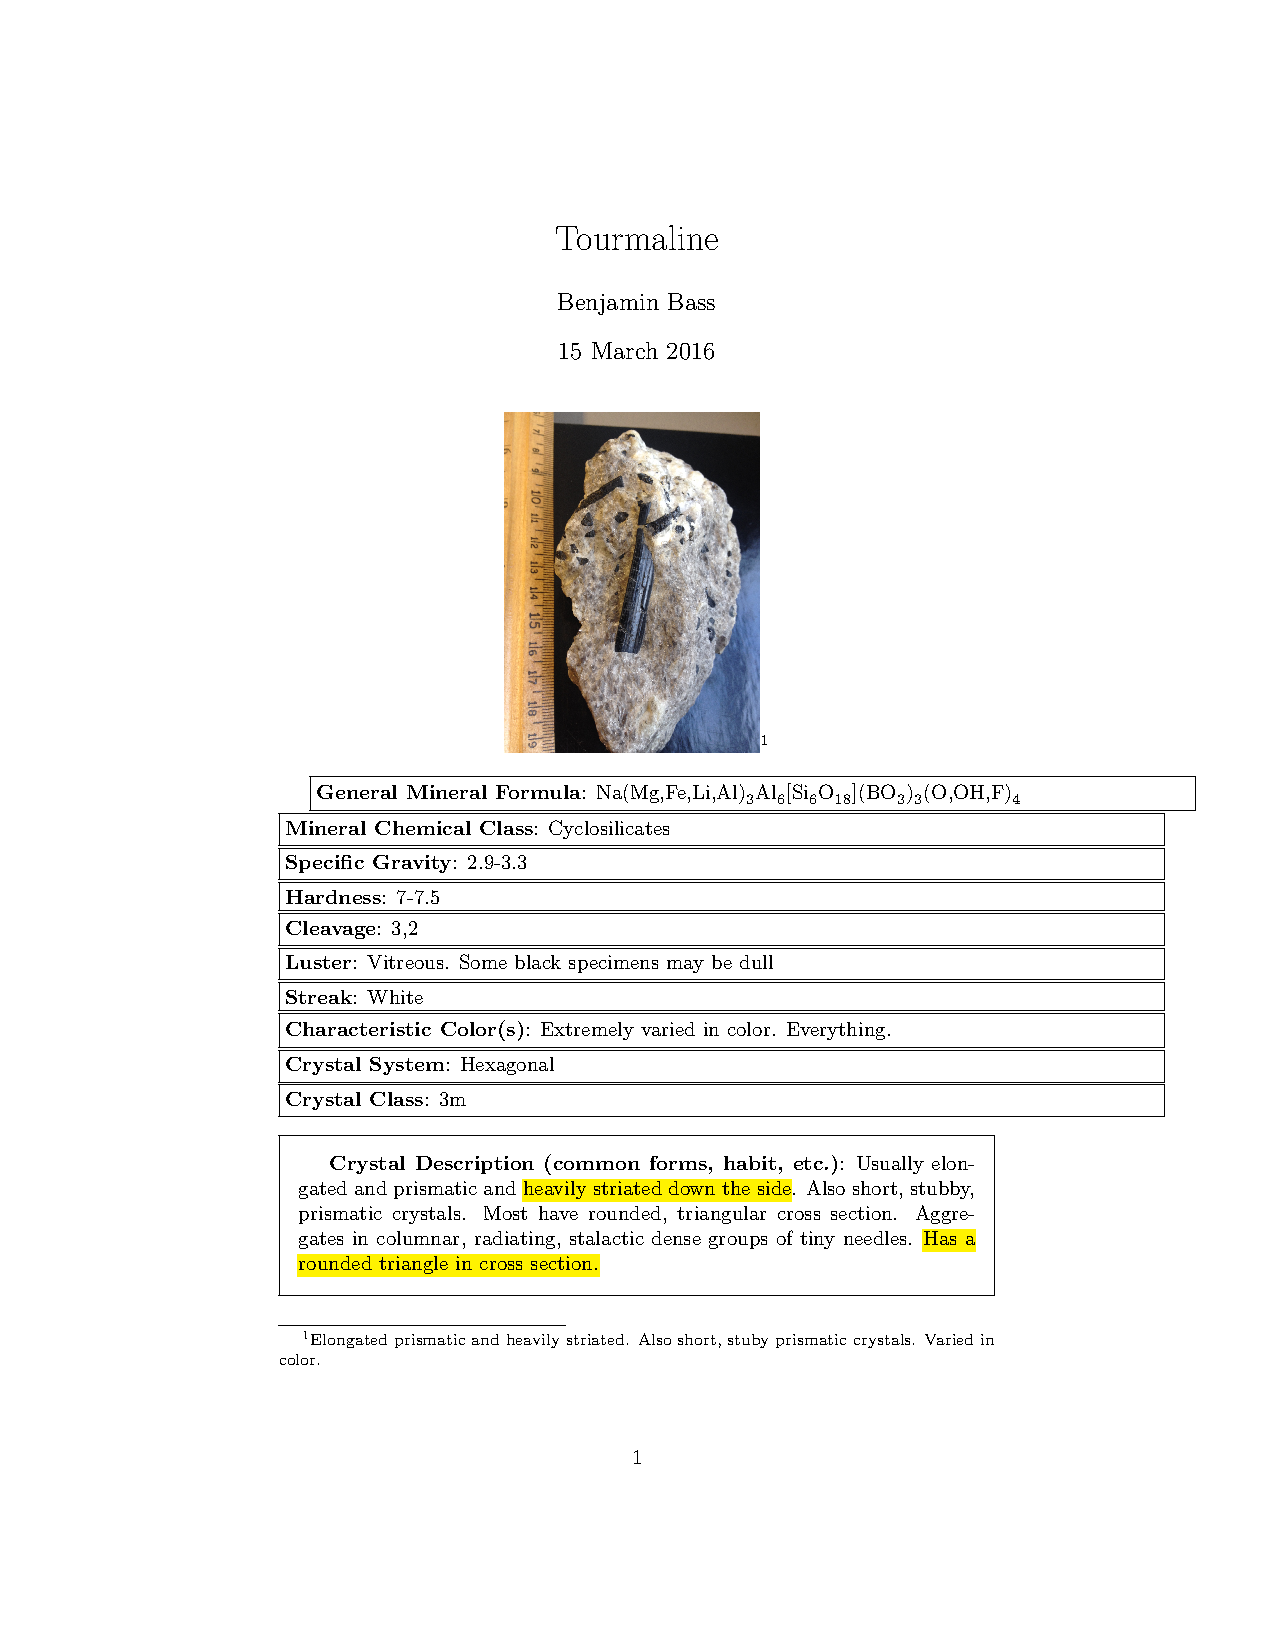
\includegraphics[scale=0.05]{tourmaline}\footnote{Elongated prismatic and heavily striated. Also short, stuby prismatic crystals. Varied in color.}
\end{center}



\framebox[15cm][l]{\textbf{General Mineral Formula}: \ce{Na(Mg\text{,}Fe\text{,}Li\text{,}Al)3Al6[Si6O18](BO3)3(O\text{,}OH\text{,}F)4} }\
\framebox[15cm][l]{\textbf{Mineral Chemical Class}: Cyclosilicates }\
\framebox[15cm][l]{\textbf{Specific Gravity}: 2.9-3.3 }\
\framebox[15cm][l]{\textbf{Hardness}: 7-7.5 }\
\framebox[15cm][l]{\textbf{Cleavage}: 3,2 }\
\framebox[15cm][l]{\textbf{Luster}: Vitreous. Some black specimens may be dull }\
\framebox[15cm][l]{\textbf{Streak}:  White}\
\framebox[15cm][l]{\textbf{Characteristic Color(s)}: Extremely varied in color. Everything. }\
\framebox[15cm][l]{\textbf{Crystal System}: Hexagonal }\
\framebox[15cm][l]{\textbf{Crystal Class}: 3m }\

\begin{framed}
  \textbf{Crystal Description (common forms, habit, etc.)}: Usually elongated and prismatic and \hl{heavily striated down the side}. Also short, stubby, prismatic crystals. Most have rounded, triangular cross section. Aggregates in columnar, radiating, stalactic dense groups of tiny needles. \hl{Has a rounded triangle in cross section.}
\end{framed}

\begin{framed}
  \textbf{Environment (where you find the material)}: Elbaite, Schorl, and Liddicoatite and almost exclusively in granite pegmatites.
\end{framed}

\begin{framed}
  \textbf{Common Mineral Associations (in samples, also consult text, notes}: Quartz, Microcline, Albite, Lepidolite, Beryl
\end{framed}

\begin{framed}
  \textbf{Scientific Usage/Significance}: None
\end{framed}

\begin{framed}
  \textbf{Industrial or Social Use/Significance}: Very popular gemstone.
\end{framed}

\begin{framed}
  \textbf{Environmental Significance}: None
\end{framed}

% Possible other Solutions
% \framebox(300,20){\minibox{\textbf{R-Sq}:For example}}

\end{document}
%%% Local Variables:
%%% mode: latex
%%% TeX-master: t
%%% End:
